%iffalse
\let\negmedspace\undefined
\let\negthickspace\undefined
\documentclass[journal,12pt,onecolumn]{IEEEtran}
\usepackage{cite}
\usepackage{amsmath,amssymb,amsfonts,amsthm}
\usepackage{algorithmic}
\usepackage{graphicx}
\usepackage{textcomp}
\usepackage{xcolor}
\usepackage{txfonts}
\usepackage{listings}
\usepackage{enumitem}
\usepackage{mathtools}
\usepackage{gensymb}
\usepackage{comment}
\usepackage[breaklinks=true]{hyperref}
\usepackage{tkz-euclide} 
\usepackage{listings}
\usepackage{gvv}                                        
%\def\inputGnumericTable{}                                 
\usepackage[latin1]{inputenc}     
\usepackage{xparse}
\usepackage{color}                                            
\usepackage{array}                                            
\usepackage{longtable}                                       
\usepackage{calc}                                             
\usepackage{multirow}
\usepackage{multicol}
\usepackage{hhline}                                           
\usepackage{ifthen}                                           
\usepackage{lscape}
\usepackage{tabularx}
\usepackage{array}
\usepackage{float}
\newtheorem{theorem}{Theorem}[section]
\newtheorem{problem}{Problem}
\newtheorem{proposition}{Proposition}[section]
\newtheorem{lemma}{Lemma}[section]
\newtheorem{corollary}[theorem]{Corollary}
\newtheorem{example}{Example}[section]
\newtheorem{definition}[problem]{Definition}
\newcommand{\BEQA}{\begin{eqnarray}}
\newcommand{\EEQA}{\end{eqnarray}}
\usepackage{float}
\usepackage{listings}
\usepackage{xcolor}
%\newcommand{\define}{\stackrel{\triangle}{=}}
\theoremstyle{remark}
\usepackage{ circuitikz }
%\newtheorem{rem}{Remark}
% Marks the beginning of the document
\begin{document}
\title{6.5.7}
\author{EE24BTECH11007 - Arnav Makarand Yadnopavit}
\maketitle
\renewcommand{\thefigure}{\theenumi}
\renewcommand{\thetable}{\theenumi}
\parindent 0px Question: Find both the maximum value and the minimum value of $3x^4 - 8x^3 + 12x^2 - 48x + 25$ on the interval \sbrak{0, 3}\\
\solution\\
\textbf{Theoretical Solution:}\\
\begin{align}
    f\brak{x}=3x^4 - 8x^3 + 12x^2 - 48x + 25 \label{eq:f}
\end{align}
Differentiating with respect to $x$ on both sides of \eqref{eq:f}
\begin{align}
    f^\prime\brak{x}=12x^3-24x^2+24x-48 \label{eq:fx}
\end{align}
Using the property that $f^\prime\brak{x}=0$ at extrema
\begin{align}
    f^\prime\brak{x}=0\\
    12x^3-24x^2+24x-48=0\\
    \brak{x-2}^3=0
\end{align}
Thus extrema exists on $x=2$.Now differentiating \eqref{eq:fx} on both sides to get $f^{\prime\prime}\brak{x}$
\begin{align}
    f^{\prime\prime}\brak{x}=36x^2-48x+24 \label{eq:f2x}
\end{align}
putting x=2 in \eqref{eq:f2x}
\begin{align}
    f^{\prime\prime}\brak{2}=72\\
    \implies f^{\prime\prime}\brak{2}>0
\end{align}
Hence minima at x=2 of value $f\brak{2}=-39$. Now checking for global maxima on boundaries
\begin{align}
    f\brak{0}=25\\
    f\brak{3}=16
\end{align}
Hence for $f\brak{x}$ in interval \sbrak{0, 3} minimum value is -39 and maximum value is 25\\ 
\textbf{Computational Solution:}\\
Using Gradient Descent to find extrema
\begin{align}
    h&=0.001\\
    x_{n+1}&=x_{n}-h\brak{f^\prime\brak{x_n}}\\
    y_{n+1}&=y_n-\brak{x_{n+1}-x_{n}}\brak{f^\prime\brak{x_n}}\\
    y_{n+1}&=y_n-\brak{x_{n+1}-x_{n}}\brak{12x_n^3-24x_n^2+24x_n-48}\\
\end{align}
We get global maxima $y\brak{0}=25$ and global minima $y\brak{2}=-39$ from the code
\begin{figure}[h]
    \centering
    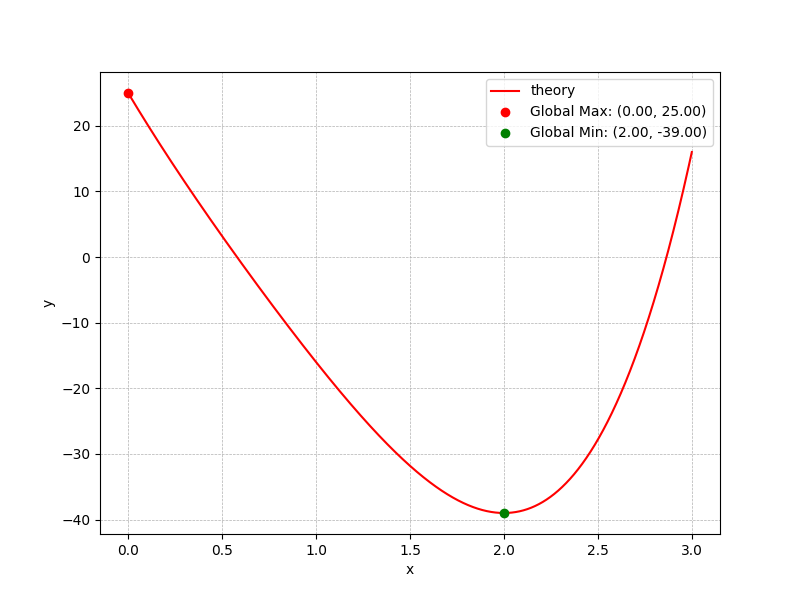
\includegraphics[width=\columnwidth]{figs/fig.png}
 \end{figure}
\end{document}
